\subsection{Impulse Response Function}
What is an impulse response function? \\
\begin{figure}[H]
    \centering
    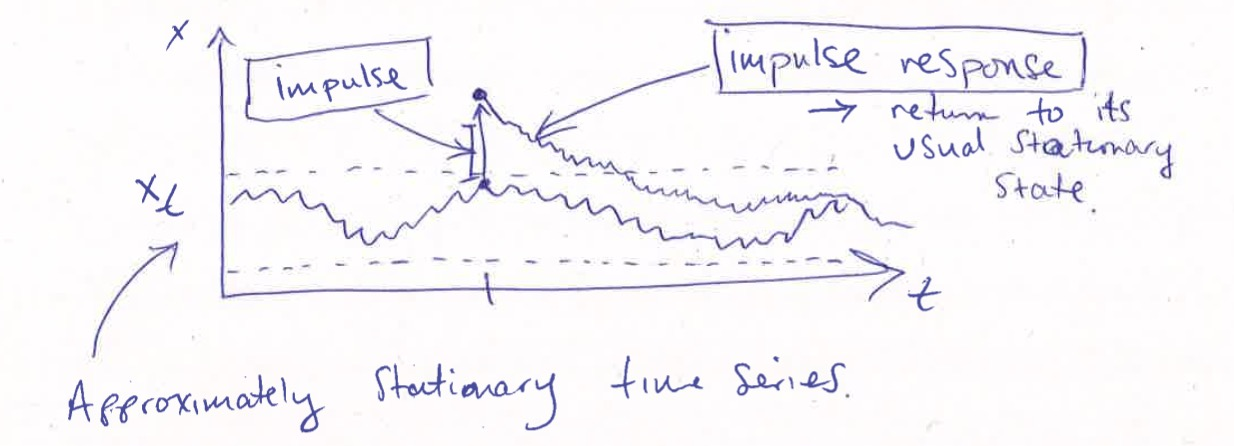
\includegraphics[width=0.8\linewidth]{images/Screenshot 2024-05-21 at 18.13.20.jpg}
    \caption{Impulse Response Function}
\end{figure}


\noindent
\rule{\linewidth}{0.4pt}
Will work towards a definition where 
\begin{align*}
    &\fbox{IRF(r)} \quad \text{is related to (or equal to)} \\
    & \frac{ d X_{t+r} }{ d \varepsilon_t }\\
\end{align*}

Suppose $X_t=\alpha + \varepsilon_t +\theta_1 \varepsilon_{t-1} + \theta_2 \varepsilon_{t-2}$ 
\begin{itemize}
    \item This is a MA(2) process with parameters $\alpha, \theta_1, \theta_2$
    \item Stationary
    \item Can define $x_t$ if you know all $\varepsilon_t$s 
    \begin{align*}
    IRF(r)&=\frac{dx_{t+r}}{d\varepsilon_t}\\
    IRF(0)&= \frac{d(\alpha+\varepsilon_t+\theta_1 \varepsilon_{t-1}+\theta_2 \varepsilon_{t-2}}{d\varepsilon_t}\\ 
    &=1\\
    IRF(1)&=\theta_1\\
    IRF(2)&=\theta_2
    \end{align*}
\end{itemize}

IRFs for more general models.
\begin{itemize}
    \item Stationary time series are almost always approximated by moving averages (MA) series.
    \item Mathematically, there is a MA($\infty$) representation of a stationary time series in many cases. 
    \item Example: AR(1) model:
    \[
    X_t = \alpha + \rho X_{t-1}+\varepsilon_t
    \]
    \begin{itemize}
        \item Invert backshift operator: $X_{t-1}=BX_t$ \[
        X_t= \alpha+\rho BX_t +\varepsilon_t
        \]\[
        \Rightarrow (1-pB)X_t=\alpha+\varepsilon_t
        \]
    \end{itemize}
    \item If $|p|<1$ its possible to invert $(1-pB)$ (why? if the roots of the "polynomial in B" are outside unit circle, then you can "divide")
    \begin{itemize}
        \item Solve $1-\rho B = 0 \longrightarrow B = \frac{1}{\rho} > 1$ if $0<\rho<1$
    \end{itemize}
\end{itemize}
\begin{align*}
    X_t= \alpha+\rho BX_t +\varepsilon_t\\  
    \Rightarrow (1-pB)X_t=\alpha+\varepsilon_t \\
    \text{if } |p|<1 \quad \text{then}\\
    (1-\rho B)^{-1} = ?
\end{align*}
Simpler example 
\begin{align*}
    \frac{1}{1-\frac{1}{4}} &= 1+\frac{1}{4} + \frac{1}{16} + \frac{1}{64} + \cdots \\
    &= \frac{4}{3}
\end{align*}
\underline{Define}: \[
(1-\rho B)^{-1}= 1+\rho B + \rho^2 B^2 + \rho^3 B^3 + \cdots
\]
Theorem: if $X_t$ is sufficiently well behaved (stationary etc.) and $|p|<1$ then \[
(1-\rho B)^{-1}X_t= (1+\rho B + \rho^2 B^2 + \rho^3 B^3)X_t
\]
and $(1-\rho B)^{-1} (1-\rho B) X_t = X_t$ (cancellation property).

\begin{align*}
    X_t &= \alpha+ \rho B X_t + \varepsilon_t\\
    (1-\rho B) X_t &= \alpha + \varepsilon_t \\
    (1-\rho B)^{-1}(1-\rho B) X_t &= (1-\rho B)^{-1} (\alpha + \varepsilon_t)\\
    \Rightarrow X_t &= \alpha + \varepsilon_t + \rho B(\alpha + \varepsilon_t)+ \rho^2 B^2(\alpha+\varepsilon_t) + \cdots
\end{align*}
The point: Now you can calculate impulse responses
\begin{align*}
    \frac{dX_t}{d\varepsilon_{t-r}} &= \frac{d}{d \varepsilon_{t-r}} \rho^r (\alpha+\varepsilon_{t-1}) \\
    &= \frac{d}{d\varepsilon_{t-r}} \rho^r \varepsilon_{t-r} \\
    &= \rho^r\\
    IRF(r) &= \rho^r
\end{align*}
$\rho^r$ measures "where $X_t$ would have been"
\begin{figure}[H]
    \centering
    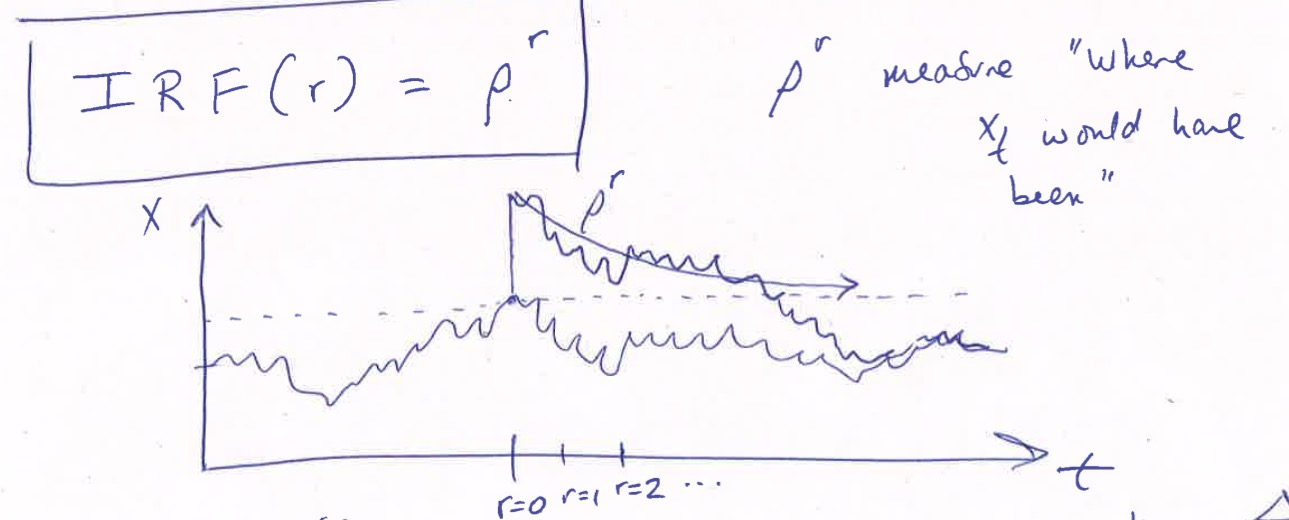
\includegraphics[width=0.75\linewidth]{images/Screenshot 2024-05-21 at 18.16.58.jpg}
\end{figure}

In ARMA(1,1)
\begin{align*}
    X_t &= \alpha + \rho X_{t-1} + \varepsilon_t + \theta \varepsilon_{t-1} \\
    (1-\rho B)X_t &= \alpha + \varepsilon_t + \theta \varepsilon_{t-1} \\
    X_t &= (1-\rho B)^{-1} (\alpha + \varepsilon_t + \theta \varepsilon_{t-1}) \\
&= 1\cdot (\alpha + \varepsilon_t + \theta \varepsilon_{t-1} + \rho B (\alpha + \varepsilon_t + \theta \varepsilon_{t-1}) + \rho^2 B^2(\alpha + \varepsilon_t + \theta\varepsilon_{t-1})\\
&\text{get IRF that way}
\end{align*}

\subsection{Multivariate Time Series}

Modeling joint dynamics of a multivariate time series.\\
\quad Most common (or basic) approach is to specify a \underline{vector autoregression} \fbox{VAR}.\\

In a bivariate case, $(x_t,y_t) $ two time series
\begin{figure}[H]
    \centering
    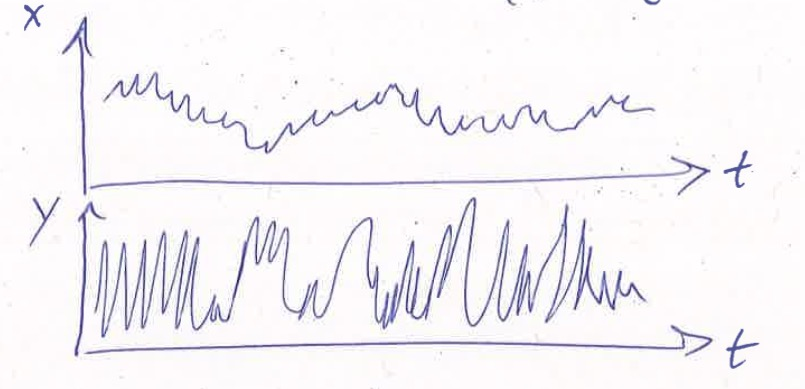
\includegraphics[width=0.75\linewidth]{images/Screenshot 2024-05-21 at 18.18.51.jpg}
\end{figure}

VAR of order 1 is a model of the form: 
\begin{align*}
    y_t&= \alpha+\rho y_{t-1} + \theta x_{t-1} + \varepsilon_t\\
    x_t&= \beta + \xi y_{t-1} + \zeta x_{t-1} + u_t
\end{align*}
Can be written in matrix notation, helpful for more than 2 time series\\
Consider $(X_{t,1}, X_{t,2})$ as a bivariate time series. \\
$(X_{t,1}, X_{t,2},\cdots,X_{t,\kappa})$ as a $\kappa$-variate time series. \\

Call the vector of observations at time $t$: $X_t$ \\
Similar for $\varepsilon_t$ \\
Then $VAR(1)$ model is written \[
    x_t= \Phi X_{t-1} + \varepsilon_t
\] \quad where $\Phi$ is a matrix

\noindent
\rule{\linewidth}{0.4pt}
\begin{align*}
    \text{If } &y_t = x_{t,1}  \quad x_t = x_{t,2} \ ,\  \Phi = \begin{pmatrix}
\rho & \theta \\
\xi & \zeta 
\end{pmatrix} \\
&\varepsilon_t = \varepsilon_{t,1}  \quad u_t = \varepsilon_{t,2} \\
\text{Then} \\
x_t&= \Phi x_{t-1}+ \varepsilon_t \Leftrightarrow \begin{matrix}
    y_t=\rho y_{t-1} + \theta x_{t-1} + \varepsilon \\
    x_t = \xi y_{t-1} + \zeta x_{t-1} + u_t
\end{matrix}
\end{align*}

Multivariate time series with notation: $X_t = \Phi X_{t-1}  +\varepsilon_t$
\begin{itemize}
    \item Can estimate $\hat{\Phi}$ with maximal likelihood
    \item IRFs - Still problems in defining them
    \begin{itemize}
        \item There are several
        \item For univariate time series we used a MA($\infty$) representation
        \item Will have to take a stand on whether $\varepsilon_{t,1}$ or $\varepsilon_{t,2}$ comes first
        \item There are other alternatives (long run restrictions, ...) 
    \end{itemize}
\end{itemize}
\[
X_t = \Phi X_{t-1} + \varepsilon_t \quad \quad X_t = \begin{pmatrix}
    X_{t,1} \\
    X_{t,2}
\end{pmatrix} ,\ \varepsilon_t = \begin{pmatrix}
    \varepsilon_{t,1}\\
    \varepsilon_{t,2}
\end{pmatrix}
\]
Several impulse response functions:
\begin{align*}
    & \frac{\partial x_{t+r, 1}}{\partial \varepsilon_{t, 1}} & \quad \frac{\partial x_{t+r, 2}}{\partial \varepsilon_{t, 1}} \\
    & \frac{\partial x_{t+r, 1}}{\partial \varepsilon_{t, 2}} & \quad \frac{\partial x_{t+r, 2}}{\partial \varepsilon_{t, 2}}
\end{align*}

\noindent
\rule{\linewidth}{0.4pt}
\noindent
What is a MA($\infty$) for a VAR?\\
Want this to facilitate calculating above 4 listed derivatives.

\begin{align*}
    & \text{Let } B X_t = X_{t-1} \text{ again.} \\
    & B = \begin{pmatrix}
    B_{1-\text{dim}} & 0 \\
    0 & B_{1-\text{dim}}
    \end{pmatrix}
\end{align*}

\[
B \begin{pmatrix}
x_{t,1} \\
x_{t,2}
\end{pmatrix}
= \begin{pmatrix}
B_{1-\text{dim}} x_{t,1} \\
B_{1-\text{dim}} x_{t,2}
\end{pmatrix}
= \begin{pmatrix}
x_{t-1,1} \\
x_{t-1,2}
\end{pmatrix}
\]

\[
(I - \Phi B) x_t = \varepsilon_t
\]

Form \((I - \Phi B)^{-1} \varepsilon_t = X_t\):

\[
X_t = I \varepsilon_t + \Phi B \varepsilon_t + (\Phi B)^2 \varepsilon_t + (\Phi B)^3 \varepsilon_t + \cdots
\]
